\documentclass[10pt,conference,compsocconf]{IEEEtran}

\usepackage{hyperref}
\usepackage{graphicx}
\usepackage{amsmath}
\usepackage{booktabs}

\begin{document}
\title{Predicting Coronary Heart Disease from Lifestyle Survey Data\\with Weighted Logistic Regression}

\author{
  Yvan B\'enon, Gr\'egoire Taillard, Jean Erard\\
  \textit{CS-433 Machine Learning, EPFL, Switzerland}
}

\maketitle

\begin{abstract}
We predict whether a person has been diagnosed with coronary heart disease
(MICHD) from 321 answers to the BRFSS health survey. The data is noisy
(missing values, special answer codes) and strongly imbalanced (8.8\% of
positive cases), so that the six basic methods seen in class reach an F1
score of at most 0.11. We decode the survey answer codes, one-hot encode the
categorical answers, add pairwise interactions between the most informative
features, and train an L2-regularized, class-weighted logistic regression with
Newton's method, whose regularization and decision threshold are tuned by
cross-validation to maximize the F1 score. The final model reaches
F1~=~0.443 (accuracy 0.882) on the AIcrowd test set. An ablation study shows
that adapting the decision rule to the class imbalance is by far the most
important ingredient.
\end{abstract}

\section{Introduction}
Cardiovascular diseases are a leading cause of death worldwide. The
Behavioral Risk Factor Surveillance System (BRFSS) is a telephone survey
of U.S.\ residents about their health and lifestyle. Given the answers of
a person, we predict $y=1$ if the person has MICHD (heart attack or
angina) and $y=-1$ otherwise. The training set contains $N=328{,}135$
people and $D=321$ features, the test set 109{,}379 people. Since only
8.8\% of the labels are positive, always predicting $-1$ gives 91\%
accuracy but is useless; we therefore optimize and report the F1 score of
the positive class, the metric of the competition. Only NumPy is used.

\section{Models and Methods}

\subsection{Evaluation protocol}
The training set is randomly split (seed 42) into a 60\% \emph{training
part} and a 40\% \emph{hold-out part}. The preprocessing and the
hyperparameters are learned on the training part only (hyperparameters by
5-fold cross-validation, CV), and Tables~\ref{tab:baselines}
and~\ref{tab:ablation} are measured on the hold-out part. The final model
is retrained on the full training set (\texttt{run.py}).

\subsection{Preprocessing}
The pipeline (\texttt{preprocessing.py}) is fitted on the training data and
applied unchanged to the other sets:
\begin{enumerate}
\item drop the 16 survey metadata features (interview date, sample ids,
  sampling weights), which do not describe the person;
\item \emph{decode the BRFSS answer codes}, with a rule deduced from the
  largest value of each feature: 7/9, 77/99, 777/999 (``don't know'',
  ``refused'') become missing; 8/88/888 (``none'') and 555 (``never'')
  become 0; frequencies coded \texttt{Pxx} (e.g.\ 203 = 3 times a week)
  are converted to times per day, which matches the variables pre-computed
  by the BRFSS (correlation 0.9999);
\item drop the features with $\geq 95\%$ missing values and the almost
  constant ones (one value in $\geq 99\%$ of the non-missing entries);
\item \emph{one-hot encode} the non-binary features with at most 10 values
  (missing counted as a value), with a reference category;
\item standardize the other features and replace missing values by 0
  (the mean); drop features with correlation $\geq 0.99$ with a previous one;
\item \emph{interactions}: add the standardized products of all pairs among
  the 30 features most correlated with the label (age, general health,
  diabetes, high blood pressure, stroke, \dots), removing constant products.
\end{enumerate}
This gives $D'=866$ features (441 without interactions).

\subsection{Baselines}
We train the six methods of \texttt{implementations.py} on the cleaned
features without interactions (some products are collinear, which makes
least squares singular): linear regression by gradient descent (GD, 100
steps, $\gamma=0.02$), by stochastic gradient descent (SGD, $10^4$ steps,
$\gamma=10^{-3}$), by the normal equations (least squares) and with an L2
penalty (ridge, $\lambda=4.6\cdot10^{-4}$ chosen by 5-fold CV on the RMSE),
and logistic regression without and with penalty ($\lambda=10^{-4}$) by
gradient descent (100 steps, $\gamma=0.1$, labels in $\{0,1\}$). The step
sizes are below the stability limits $2/L$ and $8/L$, with $L\approx49$ the
largest eigenvalue of $X^\top X/N$. All predict $1$ if
$\mathbf{x}^\top\mathbf{w}\geq 0$.

\subsection{Our model}
We minimize a class-weighted, L2-regularized logistic loss
\begin{equation}
\mathcal{L}(\mathbf{w}) = \frac{1}{N}\sum_{n=1}^{N} c_n
\log\!\left(1+e^{-y_n \mathbf{x}_n^\top \mathbf{w}}\right)
+ \lambda\|\mathbf{w}\|^2,
\end{equation}
with balanced weights $c_n = N/(2N_{y_n})$ ($N_{y_n}$: size of the class of
$n$), so that both classes have the same total weight. We use
\emph{Newton's method}: each step solves
$H\,\Delta\mathbf{w} = \nabla\mathcal{L}$ with
$H = \frac{1}{N}X^\top S X + 2\lambda I$,
$S=\mathrm{diag}(c_n\sigma_n(1-\sigma_n))$,
$\sigma_n=\sigma(\mathbf{x}_n^\top\mathbf{w})$. It converges in about 10
steps and needs no step size. A sample is classified as positive if
$\mathbf{x}^\top\mathbf{w}\geq t$.

The regularization $\lambda\in\{10^{-4},10^{-3.5},\dots,10^{-2}\}$ and the
threshold $t\in\{-2,-1.9,\dots,1.9\}$ are chosen \emph{together} by 5-fold
CV on the training part, maximizing the mean validation F1 score:
$\lambda=10^{-3}$ and $t=1.1$ (CV F1 = 0.425, Fig.~\ref{fig:threshold}).
The final model uses 15 Newton steps.

\section{Results}

\begin{table}[tbp]
  \centering
  \caption{The six basic methods on the hold-out set (threshold 0,
  cleaned features without interactions).}
  \label{tab:baselines}
  \begin{tabular}{lcc}
    \toprule
    Method & F1 & Accuracy \\
    \midrule
    Least squares GD & 0.000 & 0.911 \\
    Least squares SGD & 0.006 & 0.911 \\
    Least squares (normal equations) & 0.106 & 0.913 \\
    Ridge regression & 0.100 & 0.913 \\
    Logistic regression (GD) & 0.063 & 0.911 \\
    Reg.\ logistic regression (GD) & 0.062 & 0.911 \\
    \bottomrule
  \end{tabular}
\end{table}

\begin{table}[tbp]
  \centering
  \caption{Ablation study on the hold-out set. Newton logistic regression,
  threshold $t$ tuned by 5-fold CV unless stated otherwise.}
  \label{tab:ablation}
  \begin{tabular}{lcccc}
    \toprule
    Variant & $D'$ & $t$ & F1 & Acc. \\
    \midrule
    Basic preprocessing$^*$ & 417 & 0.9 & 0.433 & 0.866 \\
    + metadata, codes decoded & 332 & 1.0 & 0.434 & 0.874 \\
    + one-hot up to 10 values & 441 & 0.9 & 0.433 & 0.866 \\
    \textbf{+ interactions (final)} & 866 & 1.1 & 0.432 & 0.878 \\
    Final, no class weights & 866 & $-1.3$ & 0.435 & 0.876 \\
    Final, threshold $t=0$ & 866 & 0 & 0.378 & 0.760 \\
    \bottomrule
  \end{tabular}\\[1mm]
  \footnotesize{$^*$ no decoding, one-hot up to 5 values,
  $\lambda=2.15\cdot10^{-5}$ (our first submission).}
\end{table}

\begin{figure}[tbp]
  \centering
  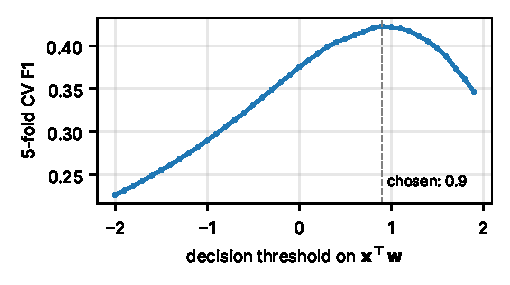
\includegraphics[width=\columnwidth]{threshold_cv}
  \vspace{-6mm}
  \caption{Mean 5-fold CV F1 score of the final model
  ($\lambda=10^{-3}$) as a function of the decision threshold $t$.}
  \label{fig:threshold}
\end{figure}

Table~\ref{tab:baselines} shows that all basic methods reach about 91\%
accuracy, the accuracy of always predicting $-1$: because of the
imbalance, almost all scores are negative and the F1 score stays below
0.11. GD and SGD are even worse than the closed-form solution, as they are
far from convergence with a stable step size.

Table~\ref{tab:ablation} shows that the decision rule is what matters:
with the default threshold the final model predicts 30\% of positives and
reaches only 0.378, while the tuned threshold gives 0.432 (+0.055).
Class weights and threshold tuning are interchangeable: without weights,
the tuned threshold ($t=-1.3$) gives the same F1 score.

The differences between the preprocessing variants on the hold-out set
(0.432--0.434) are smaller than its noise ($\approx\pm0.004$ with 11{,}500
positive samples). We therefore also compared the first and the final
pipeline with a paired 5-fold CV on the full training set (same folds, best
threshold of each fold): the final pipeline is better on all 5 folds, by
$+0.004$ F1 on average ($+0.002$ without the interactions). The test set
confirms it: our first submission obtained F1~=~0.438 (accuracy 0.869) on
AIcrowd, the final model \textbf{F1~=~0.443} (accuracy 0.882).

\section{Discussion}
The main difficulty of this dataset is the class imbalance, not the model
complexity: a linear model reaches an F1 score of 0.43 once its decision
rule is adapted, and better features only add a few thousandths. We also
tried quantile binning of the continuous features (any non-linear shape
per feature), clipping of outliers, missing-value indicators and one-hot
encoding up to 15 values, without improvement; only the interactions,
which model joint effects (e.g.\ age with diabetes), helped slightly.
Decoding the answer codes mainly makes the features meaningful and the
model smaller: most special codes were already captured by one-hot
encoding.

The model has limits. The threshold optimizes F1, which favors recall
over accuracy; a medical use could prefer another trade-off. The
preprocessing, including the choice of the interactions, is fitted once on
the training part before cross-validation, which slightly leaks
information into the validation folds; the agreement between CV, hold-out
and test scores suggests that this effect is small.

\section{Summary}
Decoding the survey answers, one-hot encoding, pairwise interactions, and
a weighted L2-regularized logistic regression trained with Newton's
method, with its regularization and threshold tuned by cross-validation
for the F1 score, raise the F1 score from at most 0.11 for the basic
methods to 0.443 on the test set. Handling the class imbalance accounts
for most of the gain. All results are reproduced by \texttt{run.py} and
\texttt{exploration.ipynb}.

\end{document}
